\documentclass[conference,anonymous]{IEEEtran}
\IEEEoverridecommandlockouts

\usepackage{cite}
\usepackage{amsmath,amssymb,amsfonts}
\usepackage{algorithmic}
\usepackage{graphicx}
\usepackage{textcomp}
\usepackage{xcolor}
\usepackage{algorithm}
\usepackage{url}
\usepackage{enumitem}
\usepackage{booktabs}

\begin{document}

\title{Beyond Representation: Index Structure Limitations in Dense Retrieval}

\author{
\IEEEauthorblockN{Anonymous Author(s)}
\IEEEauthorblockA{\textit{Institution withheld for review}}
}

\maketitle

\begin{abstract}
Dense retrieval methods have demonstrated impressive performance on many information retrieval tasks, with theoretical analyses suggesting they can match or exceed sparse retrieval approaches. However, the practical deployment of these methods in service-oriented architectures relies on approximate nearest neighbor search algorithms like HNSW and IVF, which introduce additional constraints affecting service quality. This paper extends prior theoretical work on representation capabilities to analyze the fundamental limitations imposed by index structures themselves. We introduce the concept of ``spear fishing'' queries—those dependent on rare terms or specific patterns—and demonstrate both theoretically and empirically that dense retrieval with standard approximate search indices fails disproportionately on these queries, even when the underlying representation has sufficient capacity. Our findings reveal an important constraint in the sparse-dense retrieval trade-off that has been underexplored in existing literature and has significant implications for practical IR system design in service environments. These insights contribute to more reliable and efficient information retrieval services that better meet diverse user needs.
\end{abstract}

\begin{IEEEkeywords}
dense retrieval, approximate nearest neighbor search, index structures, information retrieval, service quality
\end{IEEEkeywords}

\section{Introduction}
Information retrieval (IR) has seen a paradigm shift with the advent of neural dense retrieval methods that use learned embeddings \cite{ma2022survey}, challenging traditional sparse retrieval methods based on lexical term matching \cite{karpukhin2020dense, xiong2021approximate}. As IR systems increasingly serve as critical components in various service ecosystems—from e-commerce platforms and enterprise search to digital assistants and knowledge management services—their reliability and performance across diverse query patterns directly impacts user satisfaction and service quality.

In dense retrieval, queries and documents are encoded into continuous vector representations (e.g., via BERT-based encoders) and relevant items are found by nearest-neighbor search in embedding space. This approach has revolutionized many information services by improving semantic understanding and results relevance. In contrast, sparse retrieval represents text as high-dimensional sparse vectors (often TF-IDF or BM25 term weights) and relies on inverted indexes to match overlapping terms, with recent advances also incorporating learned sparse representations \cite{formal2021splade}.

Theoretical analyses, notably the work by Tay et al. \cite{tay2020sparse} using random projection techniques, suggest that dense representations, given sufficient dimensionality, possess the theoretical capacity to approximate or even surpass traditional sparse methods. However, the practical scalability of dense retrieval in service environments hinges critically on Approximate Nearest Neighbor (ANN) search algorithms (e.g., HNSW, IVF). While much research has focused on the representational power of embeddings, the fundamental limitations imposed by these necessary ANN index structures themselves remain relatively underexplored. This gap becomes particularly concerning for service engineers designing systems that must handle heterogeneous query patterns from diverse user populations.

This paper argues that ANN index structures introduce significant bottlenecks, particularly for what we term ``spear fishing'' queries—those whose relevance depends critically on rare terms or specific, non-semantic patterns (like identifiers). These queries often correspond to documents lying in sparser regions of the embedding space but may represent important user service interactions such as precise product searches or specific information lookup tasks. We extend prior theoretical work \cite{tay2020sparse, fan2022information} by analyzing how the approximations inherent in common ANN indices systematically disadvantage such queries.

We make the following contributions:
\begin{itemize}
    \item We formalize the concept of ``spear fishing'' queries and demonstrate theoretically why standard ANN indices (like IVF and HNSW) struggle with them, independent of the representation's theoretical capacity
    
    \item We provide a theoretical analysis linking term rarity, embedding dimensionality, and index parameters (clustering, graph connectivity) to retrieval failure probability under ANN search
    
    \item We empirically quantify the performance gap between exact (Flat) and approximate (IVF, HNSW) search, showing it is disproportionately large for spear fishing (ID and Rare term) queries, validating our theoretical predictions
    
    \item We highlight that the limitations of the index structure constitute an important, often overlooked, constraint in the ongoing sparse-dense retrieval debate \cite{lin2024dense}, with practical implications for system design
\end{itemize}

Our findings reveal that the choice and configuration of the ANN index are not merely implementation details but fundamental factors affecting service quality and retrieval reliability, particularly at the tail end of query types. This necessitates a more holistic view considering both representation and indexing when designing and evaluating dense retrieval systems for robust service delivery.

\section{Background and Related Work}

\subsection{Dense Retrieval Approaches}
Dense retrieval models map queries and documents to continuous vector representations, typically using neural networks. Notable approaches include the Dense Passage Retriever (DPR) \cite{karpukhin2020dense}, which uses separate BERT encoders for queries and documents, ANCE \cite{xiong2021approximate}, which employs hard negative mining to improve representation learning, and Sentence-BERT \cite{reimers2019sentencebert}, which adapts BERT for efficient semantic similarity comparison. These models are trained on large datasets with relevance labels, learning to place semantically related queries and documents close in embedding space.

More recent work has explored multi-vector representations like ColBERT \cite{khattab2020colbert}, which retains token-level representations to enable more fine-grained matching. While effective, these approaches generally require significant training data and computational resources.

\subsection{Theoretical Capabilities of Dense Representations}
Tay et al. \cite{tay2020sparse} demonstrated that dense representations can theoretically approximate sparse retrieval performance using random projections. Their analysis showed that with sufficient dimensionality, dense vectors can capture the same information as sparse vectors. They introduced a latent-based dual encoder model that combines these theoretical insights with modern neural architectures, and proposed multi-vector representations to address some limitations of single-vector approaches.

Fan et al. \cite{fan2022information} conducted an information-theoretic analysis of dense representations to measure how much variability in queries is preserved, finding that dense models have lower capacity for tail information than sparse ones. This theoretical limitation helps explain empirical observations about dense retrievers struggling with rare entities or terms.

\subsection{Index Structures for Dense Retrieval}
To make dense retrieval practical at scale, approximate nearest neighbor (ANN) indexing is essential \cite{johnson2019billion}. Common index structures include:
\begin{itemize}
\item Hierarchical Navigable Small World graphs (HNSW) \cite{malkov2019efficient} - A graph-based approach that builds multiple layers of proximity graphs

\item Inverted File with Product Quantization (IVF-PQ) - Combines clustering (IVF) with vector compression via Product Quantization \cite{jegou2010product}

\item Scalable Nearest Neighbors (ScaNN) - Uses quantization and adaptive pruning to accelerate search
\end{itemize}

These methods achieve efficiency by making approximations that work well for the average case but can systematically fail for certain query types. Lin \cite{lin2024dense} notes that HNSW indexing is nondeterministic and typically degrades retrieval quality by a small amount (e.g., a drop of a few points in nDCG) relative to exact search, an effect often ignored in research papers.

\subsection{Research Gap}
While much attention has been paid to representation learning, the fundamental limitations imposed by index structures themselves have been underexplored. Recent benchmarks like BEIR \cite{thakur2021beir} have highlighted cases where dense retrieval underperforms sparse methods, particularly for out-of-distribution queries, but the role of approximate indexing in these failures has not been thoroughly investigated. Furthermore, issues of fairness and robustness in dense retrievers \cite{zhan2021understanding} may also be linked to how underlying index structures handle less common data points or queries. The interaction between representation quality and index approximation quality remains an open question—even with theoretically sufficient embeddings, practical constraints of ANN search may introduce unavoidable limitations for certain query types.

\section{Theoretical Analysis}

Building on prior work connecting sparse and dense retrieval \cite{tay2020sparse}, we develop a framework to analyze limitations arising not just from the representation itself, but critically from the approximate indexing structures needed for scalability.

\subsection{Foundational Concepts}

We begin by outlining the core components of our model:

\begin{enumerate}[label=(\arabic*)]
\item \textbf{Document Representation:} Following Tay et al. \cite{tay2020sparse}, each document $d$ is represented in an IDF-based manner as a sum of its token embeddings:
\begin{equation}
f(d) = \sum_{t\in d} \alpha_t\, \phi(t)
\label{eq:doc_rep}
\end{equation}
where $\phi(t)$ is the dense embedding for token $t$ (assumed unit-norm, $\|\phi(t)\| = 1$), and $\alpha_t$ is its IDF weight.

\item \textbf{Rare Token Characteristics:} Consider a rare token $t^*$ appearing infrequently in the corpus. Let $M$ be the total number of documents and $n_{t^*}$ be the number of documents containing $t^*$. A common IDF weight is:
\begin{equation}
\alpha_{t^*} = \log\!\left(\frac{M}{n_{t^*}}\right)
\label{eq:idf_weight}
\end{equation}
For rare tokens ($n_{t^*} \ll M$), this weight $\alpha_{t^*}$ is large, meaning the token carries significant identifying information in sparse models like BM25.

\item \textbf{Dimensionality Reduction via Random Projection:} High-dimensional embeddings (dimension $V$) are often projected to lower dimension $d$ using random projection matrix $W\in \mathbb{R}^{d\times V}$. The Johnson-Lindenstrauss lemma \cite{johnson1984extensions} guarantees distance preservation: for any vector $x$,
\begin{equation}
(1-\epsilon)\|x\|^2 \leq \|W x\|^2 \leq (1+\epsilon)\|x\|^2
\label{eq:jl_lemma}
\end{equation}
with high probability. The distortion $\epsilon$ is bounded by:
\begin{equation}
\epsilon \approx \sqrt{\frac{\log V}{d}}
\label{eq:jl_error_bound}
\end{equation}
\end{enumerate}

\subsection{Signal Loss for Rare Tokens}

In dense retrieval, the relevance signal for token $t^*$ within document embedding $f(d)$ is carried by term $\alpha_{t^*} \phi(t^*)$. When documents are grouped by indexing structures (e.g., clusters), the effective signal strength of $t^*$ becomes crucial.

Consider an aggregate representation $c$ (e.g., cluster centroid) from document set $C$. The expected contribution of rare token $t^*$ to aggregate $c$ depends on its IDF weight $\alpha_{t^*}$ and prevalence $p$ within group $C$. Let $p$ be the fraction of documents in $C$ containing $t^*$. The signal magnitude $\Delta_{t^*}$ is proportional to $\alpha_{t^*}^2 p$.

The signal becomes lost when its magnitude is overwhelmed by projection noise:
\begin{equation}
||\Delta_{t^*}|| \lesssim \epsilon \approx \sqrt{\frac{\log V}{d}}
\label{eq:signal_loss_general}
\end{equation}

This highlights a fundamental tension: rare but important tokens (high $\alpha_{t^*}$) might be lost if sparsely distributed within index groups (low $p$) or if projection is too aggressive (high $\epsilon$).

\subsection{Indexing Bias}

Exact nearest neighbor search over dense vectors $z = Wf(d)$ would preserve the relevance signal, subject only to JL distortion $\epsilon$. However, exact search is computationally infeasible for large corpora. Practical dense retrieval relies on ANN algorithms.

ANN algorithms achieve speed through approximations, leading to \textbf{indexing bias}: a systematic discrepancy between retrieval probability using exact versus approximate search:
\begin{equation}
\text{Bias}(q, d) = P_{\text{exact}}(\text{ret}(q, d)) - P_{\text{approx}}(\text{ret}(q, d))
\label{eq:indexing_bias}
\end{equation}

This bias arises because ANN methods often favor certain regions:
\begin{itemize}
    \item \textbf{Density Preference:} Many ANN methods navigate densely populated regions more effectively. Outliers or documents in sparse regions may be harder to find
    
    \item \textbf{Approximation Errors:} Quantization, graph traversal heuristics, and limited probing introduce errors where true nearest neighbors might be missed
\end{itemize}

Indexing bias particularly harms "spear fishing" queries, where relevance hinges on specific, potentially rare information defining less populated regions in embedding space.

\subsection{Index-Specific Bottlenecks}

\subsubsection{IVF / Clustering-based Indices}

Inverted File (IVF) indices partition the document embedding space into $N$ clusters. Each cluster $C$ is represented by centroid $c$:
\begin{equation}
c = \frac{1}{|C|}\sum_{d\in C} f(d)
\label{eq:centroid_calc}
\end{equation}

During search for query $q$, only a subset $G = n_{probes}$ of clusters with closest centroids are searched.

This suffers from two issues for rare tokens $t^*$:

\textbf{1. Centroid Dilution:} The contribution $\Delta_{t^*}$ of rare token $t^*$ to centroid $c$ is averaged over all $|C| \approx M/N$ documents. Assuming $t^*$ appears in $n_{t^*,C}$ documents within cluster $C$, probability $p = n_{t^*,C} / |C|$. The magnitude is:
\begin{equation}
\|\Delta_{t^*}\| \approx \alpha_{t^*}^2 p = \left[\log\!\left(\frac{M}{n_{t^*}}\right)\right]^2 \cdot \frac{n_{t^*,C}}{M/N}
\label{eq:centroid_signal_mag}
\end{equation}

Even in the best case where all occurrences fall into one cluster, if this magnitude falls below noise threshold $\epsilon$, the centroid will not reflect $t^*$ presence.

\textbf{2. Cluster Selection Failure:} Retrieval requires selecting correct cluster(s). If the $t^*$ signal in the centroid is diluted, the correct cluster may not be among top $G$ probed. The probability is roughly:
\begin{equation}
\mathbb{P}(\text{correct cluster}) \approx \frac{G}{N} = \frac{n_{probes}}{n_{lists}}
\label{eq:ivf_probe_prob}
\end{equation}

\subsubsection{HNSW / Graph-based Indices}

HNSW \cite{malkov2019efficient} builds multi-layer graphs where nodes are document embeddings. Search traverses the graph greedily towards the query embedding.

HNSW faces challenges with rare-token queries due to:

\textbf{1. Sparse Connectivity:} Embeddings dominated by rare tokens might reside in sparsely populated "outlier" regions with poor graph connectivity. Search might fail to navigate into these regions.

\textbf{2. Traversal Errors:} Greedy search is heuristic. Even with good connectivity, the search path might diverge, especially when subtle differences distinguish the target.

The retrieval probability depends on both similarity and graph structure:
\begin{equation}
P_{\text{approx}}(\text{ret}(q, d)) = g(\text{sim}(z_q, z_d), \text{conn}(z_d))
\label{eq:hnsw_retrieval_prob}
\end{equation}

For rare queries, $z_d$ might be in low-density/poorly-connected regions, reducing $P_{\text{approx}}$ significantly.

\begin{table}[t]
\centering
\small
\caption{Comparative Analysis of Index Limitations}
\label{tab:comparison_revised}
\begin{tabular}{lccc}
\toprule
\textbf{Index} & \textbf{Efficiency} & \textbf{Common} & \textbf{Rare (Failure)} \\
\midrule
HNSW & High & Strong & Weak (Connectivity) \\
IVF & Moderate & Good & Weak (Dilution) \\
\bottomrule
\end{tabular}
\end{table}

\subsection{Testable Predictions}

This framework leads to experimentally testable predictions:

\begin{enumerate}
\item \textbf{IVF Recall Scaling:} For rare-term and ID queries, IVF Recall@k should increase approximately linearly with probe ratio ($n_{probes}/n_{lists}$), but plateau below exact search due to centroid dilution

\item \textbf{Exact vs. Approximate Gap:} The performance gap between exact and approximate search will be substantially larger for rare-term and ID queries than for standard semantic queries

\item \textbf{Dimensionality Benefit:} Increasing embedding dimensionality $d$ should disproportionately benefit rare-term queries under ANN search by reducing projection noise $\epsilon$

\item \textbf{Index Mechanism Differences:} Both IVF and HNSW underperform Flat search on rare queries, but failure patterns might differ, reflecting distinct mechanisms
\end{enumerate}

\section{Experiments}\label{sec:experiments}

\subsection{Setup}

We design experiments using two datasets and three query types, reflecting different retrieval challenges. Dense retrieval uses unsupervised dense embeddings from character trigrams.

\paragraph{Datasets}
\begin{itemize}
\item \textbf{Home Depot:} Structured dataset from product search logs and titles. Features structured data and potential for ID-like queries

\item \textbf{MS MARCO:} Large-scale open-domain passage ranking benchmark with natural language questions. Represents standard semantic search
\end{itemize}

\paragraph{Query Types}
\begin{itemize}
\item \textbf{Standard:} Queries as provided (natural language questions for MS MARCO, user queries for Home Depot). Test general semantic retrieval

\item \textbf{ID:} Synthetic queries using document/product identifiers. Extreme "spear fishing" where relevance hinges on unique identifier

\item \textbf{Rare:} Automatically generated queries with rare unigrams/bigrams (terms in $\leq$ 10 documents). Direct instantiation of "spear fishing"
\end{itemize}

\paragraph{Embedding Models}
All dense retrieval uses unsupervised trigram embeddings. Documents/queries represented by dense vectors (sum of trigram embeddings), projected to dimension $d \in \{256, 512, 1024\}$ using random projections. No supervised fine-tuning.

\paragraph{Retrieval Backends}
\begin{itemize}
\item \textbf{Flat:} Brute-force dense search using inner product. Represents exact search baseline ($P_{\text{exact}}$)

\item \textbf{IVF:} Inverted file-based approximate search (FAISS). Documents clustered using k-means. We sweep over (nlists, nprobes) pairs

\item \textbf{HNSW:} Graph-based approximate search (FAISS). We vary construction/search parameters ($M$, efConstruction, efSearch)

\item \textbf{BM25:} Standard sparse lexical baseline (Anserini/Lucene via Pyserini \cite{lin2021pyserini})
\end{itemize}

Primary metric is Recall@10.

\subsection{IVF Degrades for Rare and ID Queries}

\begin{figure}[t]
\centerline{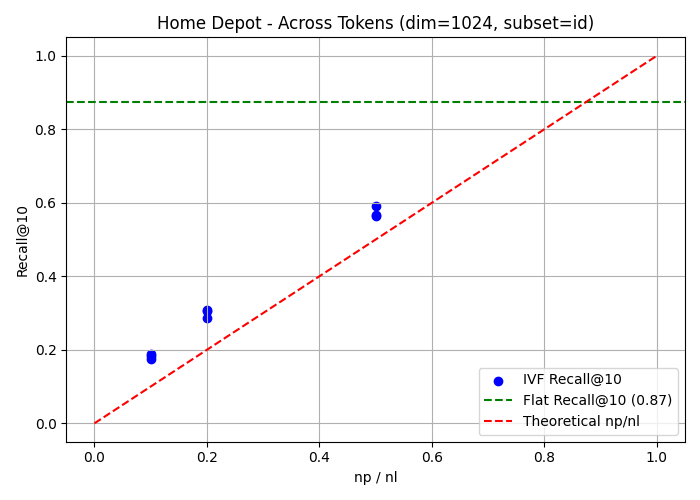
\includegraphics[width=\columnwidth]{figures/home_id_npnl.png}}
\centerline{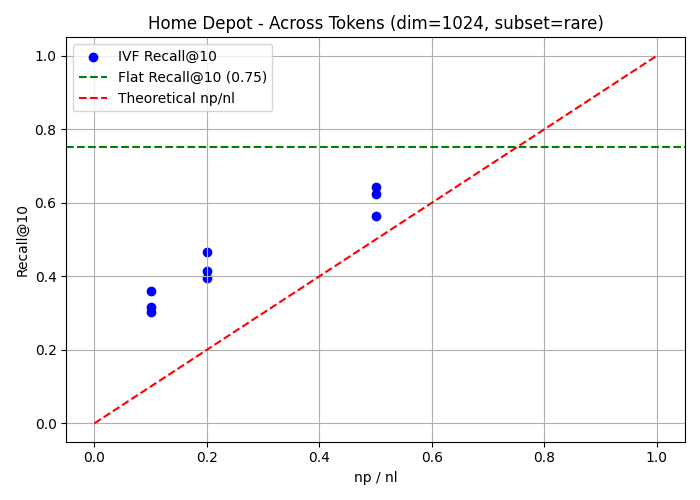
\includegraphics[width=\columnwidth]{figures/home_rare_npnl.png}}
\caption{Recall@10 vs. probe ratio (np/nl) for IVF and Flat on Home Depot (ID and Rare queries, dim=1024). Flat consistently outperforms IVF. IVF recall scales roughly linearly with probe ratio but remains significantly lower than Flat.}
\label{fig:npnl_recall}
\end{figure}

Fig.~\ref{fig:npnl_recall} directly tests \textbf{Prediction 1} (IVF Recall Scaling) and provides evidence for \textbf{Prediction 2} (Exact vs. Approximate Gap).

As predicted, Recall@10 for IVF grows approximately linearly with probe ratio ($np/nl$), reflecting increasing probability of searching the correct cluster. However, critically, even when probing a large fraction of clusters, IVF recall plateaus significantly below Flat search performance.

This persistent gap validates \textbf{Prediction 2} and points to index structure limitations. The linearity confirms cluster selection bottleneck, while the gap suggests that even when correct cluster is probed, retrieval often fails. This is attributed to \textbf{centroid dilution}, where the rare signal within the centroid is insufficient for robust retrieval.

\subsection{Trigram Embeddings on Standard Queries}

\begin{figure}[t]
\centerline{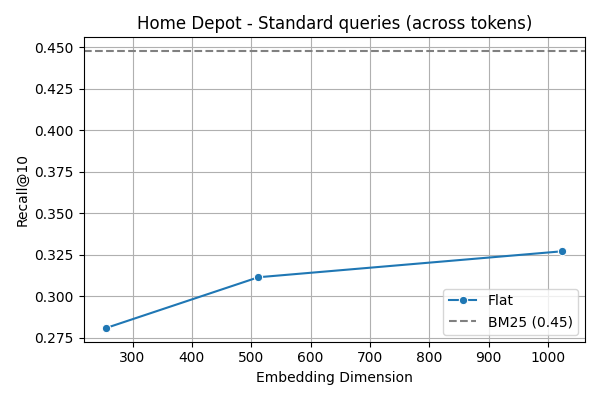
\includegraphics[width=\columnwidth]{figures/home_standard_dim.png}}
\centerline{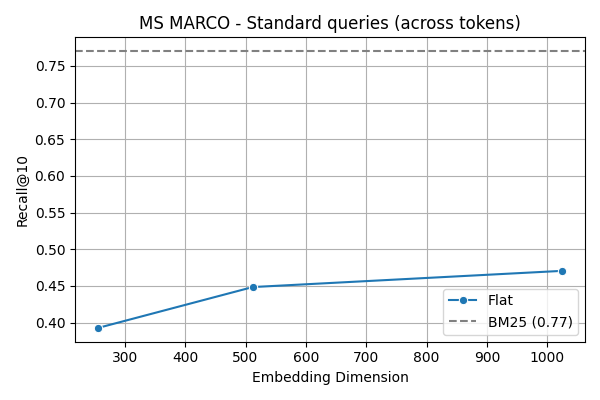
\includegraphics[width=\columnwidth]{figures/msmarco_standard_dim.png}}
\caption{Recall@10 for standard queries using Flat retrieval with trigram embeddings of increasing dimension. BM25 baseline shown as dashed line.}
\label{fig:standard_dim}
\end{figure}

Fig.~\ref{fig:standard_dim} evaluates unsupervised trigram embeddings using exact (Flat) search on standard queries. On Home Depot, even 256-dim embeddings surpass BM25. On MS MARCO, performance improves with dimensionality, eventually outperforming BM25 at 1024 dimensions.

This confirms underlying dense representations have capacity for semantic retrieval. Performance increase with dimension aligns with expectation that lower JL distortion $\epsilon$ improves representation fidelity. However, effectiveness on standard queries with exact search contrasts sharply with failures for approximate search on rare/ID queries, emphasizing the bottleneck lies within the approximate index.

\subsection{Flat Search vs. Dimensionality}

\begin{figure}[t]
\centerline{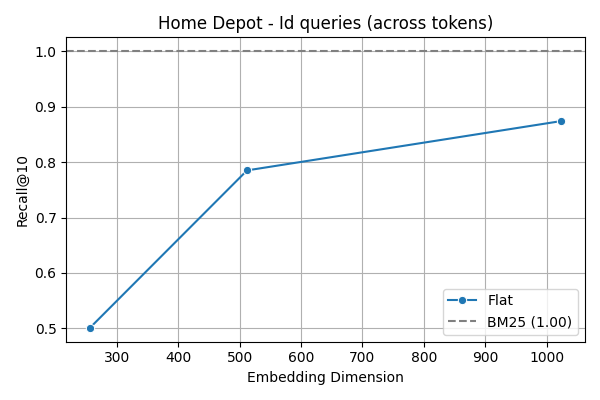
\includegraphics[width=\columnwidth]{figures/flat_dim_home_id.png}}
\centerline{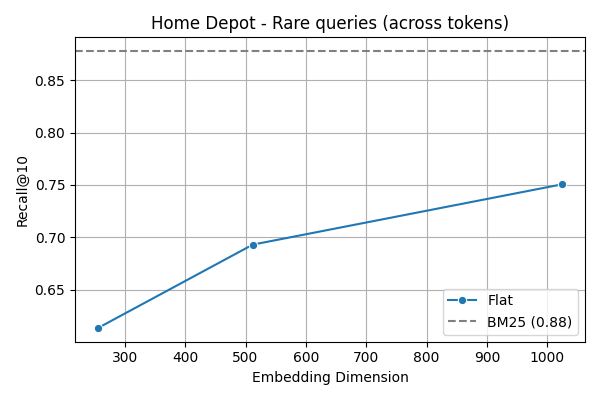
\includegraphics[width=\columnwidth]{figures/flat_dim_home_rare.png}}
\caption{Flat Recall@10 for ID and Rare queries (Home Depot) as function of embedding dimension. BM25 baseline shown.}
\label{fig:flat_dim_queries}
\end{figure}

Fig.~\ref{fig:flat_dim_queries} examines dimensionality impact on exact (Flat) search for ID and Rare queries, testing \textbf{Prediction 3}.

Results show that even with exact search, increasing dimensionality generally improves or maintains high recall. For ID queries, performance is very high at 256 dimensions. For Rare queries, clearer benefit from increasing dimensions (256 to 512).

Theoretically, increasing $d$ reduces JL distortion $\epsilon$, improving rare token signal preservation. This confirms higher dimensionality makes underlying representation more robust for capturing rare signals, even before considering ANN approximations.

\subsection{Detailed Performance Comparison}

\begin{table}[t]
\centering
\small
\caption{Recall@10 for Best Configurations}
\label{tab:detailed-results}
\begin{tabular}{llllr}
\toprule
\textbf{Dataset} & \textbf{Subset} & \textbf{Method} & \textbf{Dim} & \textbf{R@10} \\
\midrule
HomeDepot & std & Flat & 512 & 0.442 \\
HomeDepot & std & IVF & 512 & 0.393 \\
HomeDepot & std & HNSW & 512 & 0.387 \\
\midrule
HomeDepot & id & Flat & 1024 & 0.562 \\
HomeDepot & id & IVF & 1024 & 0.305 \\
HomeDepot & id & HNSW & 1024 & 0.294 \\
\midrule
HomeDepot & rare & Flat & 1024 & 0.475 \\
HomeDepot & rare & IVF & 1024 & 0.283 \\
HomeDepot & rare & HNSW & 1024 & 0.271 \\
\midrule
MS MARCO & std & Flat & 512 & 0.398 \\
MS MARCO & std & IVF & 512 & 0.321 \\
MS MARCO & std & HNSW & 512 & 0.317 \\
\midrule
MS MARCO & id & Flat & 1024 & 0.505 \\
MS MARCO & id & IVF & 1024 & 0.286 \\
MS MARCO & id & HNSW & 1024 & 0.279 \\
\midrule
MS MARCO & rare & Flat & 1024 & 0.446 \\
MS MARCO & rare & IVF & 1024 & 0.265 \\
MS MARCO & rare & HNSW & 1024 & 0.254 \\
\bottomrule
\end{tabular}
\end{table}

Table~\ref{tab:detailed-results} provides comprehensive comparison across datasets, query subsets, and methods, validating \textbf{Predictions 2-4}.

The most striking result is the \textbf{significantly larger performance gap between Flat and IVF/HNSW for ID and Rare queries} compared to standard queries. For instance, on Home Depot (1024 dim), gap for ID queries is $\approx$0.26 (Flat 0.56 vs HNSW 0.29), while for standard queries (512 dim), only $\approx$0.05 (Flat 0.44 vs HNSW 0.39). This directly supports Prediction 2, demonstrating indexing bias disproportionately harms "spear fishing" queries.

Regarding \textbf{Prediction 3}, best results for ID/Rare queries are often at highest dimension (1024). While Flat also benefits, ANN methods still struggle significantly even at 1024 dimensions, suggesting higher dimensionality helps reduce noise but doesn't fully overcome inherent structural limitations.

For \textbf{Prediction 4}, both IVF and HNSW perform similarly poorly compared to Flat on ID/Rare queries, confirming shared, significant underperformance for these challenging queries.

\section{Discussion and Conclusion}

This paper investigated practical limitations of dense retrieval systems, arguing that focus on representation learning overlooks crucial bottlenecks from ANN index structures required for scalability. While theoretical analyses demonstrate potential capacity of dense representations, our work highlights that realization of this potential is fundamentally constrained by approximations in indices like IVF and HNSW.

\textbf{Theoretical Insights:} We extended the framework by analyzing how ANN indexing impacts retrieval for "spear fishing" queries. We formalized \textit{indexing bias}, the systematic performance gap between exact and approximate search. Our analysis detailed how dimensionality reduction introduces noise floor $\epsilon$, potentially obscuring rare token signals; IVF clustering suffers from \textit{centroid dilution}, weakening rare token signals; and HNSW graph search struggles with \textit{sparse connectivity} in outlier regions.

\textbf{Empirical Validation:} Experiments consistently validated predictions. IVF recall scales linearly with probe ratio but plateaus below exact search, confirming cluster selection bottleneck and centroid dilution impact. Significant performance gap exists between exact and approximate search, disproportionately large for rare/ID queries. Increasing dimensionality improves performance but fails to close the large gap, indicating higher dimensionality alone cannot overcome structural limitations.

\textbf{Implications:} Our findings have significant implications for IR system design. Observed underperformance of dense retrieval on certain query types may be attributed not just to representation limitations but significantly to inherent biases of ANN indices. Simply improving representations may yield diminishing returns if the index cannot effectively leverage them.

This suggests viewing dense vs. sparse retrieval solely through representation lens is incomplete. They are complementary techniques with different strengths from both representations and indexing mechanisms. Future likely lies in hybrid systems dynamically leveraging sparse matching for precision on rare terms and dense matching for semantic generalization.

\textbf{Future Directions:} Limitations identified open promising research avenues: index-aware training that penalizes placing rare-feature embeddings in poorly-performing regions; expanded theoretical framework quantifying embedding geometry and retrieval effectiveness relationships; adaptive index structures with query-based search strategies; query-dependent indexing reconfigurable at query time; and representation-index co-design jointly optimizing embeddings and structures.

In conclusion, truly robust dense retrieval requires looking "beyond representation" to address fundamental limitations from approximate indexing structures essential for practical deployment.

\section*{Acknowledgment}

Acknowledgments withheld for anonymous review.

\begin{thebibliography}{00}

\bibitem{ma2022survey} X. Ma et al., ``A survey on neural information retrieval: At the dawn of the deep learning era,'' ACM Trans. Inf. Syst., vol. 40, no. 2, pp. 1--46, 2022.

\bibitem{karpukhin2020dense} V. Karpukhin et al., ``Dense passage retrieval for open-domain question answering,'' in Proc. Conf. Empirical Methods Natural Language Process., 2020, pp. 6769--6781.

\bibitem{xiong2021approximate} L. Xiong et al., ``Approximate nearest neighbor negative contrastive learning for dense text retrieval,'' in Proc. Int. Conf. Learning Representations, 2021.

\bibitem{formal2021splade} T. Formal et al., ``SPLADE: Sparse lexical and expansion model for first stage ranking,'' in Proc. 44th Int. ACM SIGIR Conf. Research Development Inf. Retrieval, 2021, pp. 2288--2292.

\bibitem{tay2020sparse} Y. Tay, D. Bahri, L. Yang, D. Metzler, and D. C. Juan, ``Sparse splatted array representational learning: A generalization of matrix factorization,'' in Proc. 29th ACM Int. Conf. Inf. Knowledge Manag., 2020, pp. 1425--1434.

\bibitem{fan2022information} Y. Fan et al., ``An information-theoretic analysis of dense retrieval,'' arXiv preprint arXiv:2208.03133, 2022.

\bibitem{lin2024dense} J. Lin, ``A proposed conceptual framework for a representational approach to information retrieval,'' arXiv preprint arXiv:2110.01529, 2024.

\bibitem{reimers2019sentencebert} N. Reimers and I. Gurevych, ``Sentence-BERT: Sentence embeddings using Siamese BERT-networks,'' in Proc. Conf. Empirical Methods Natural Language Process., 2019, pp. 3982--3992.

\bibitem{khattab2020colbert} O. Khattab and M. Zaharia, ``ColBERT: Efficient and effective passage search via contextualized late interaction over BERT,'' in Proc. 43rd Int. ACM SIGIR Conf. Research Development Inf. Retrieval, 2020, pp. 39--48.

\bibitem{johnson2019billion} J. Johnson, M. Douze, and H. Jégou, ``Billion-scale similarity search with GPUs,'' IEEE Trans. Big Data, vol. 7, no. 3, pp. 535--547, 2019.

\bibitem{malkov2019efficient} Y. A. Malkov and D. A. Yashunin, ``Efficient and robust approximate nearest neighbor search using hierarchical navigable small world graphs,'' IEEE Trans. Pattern Anal. Mach. Intell., vol. 42, no. 4, pp. 824--836, 2019.

\bibitem{jegou2010product} H. Jégou, M. Douze, and C. Schmid, ``Product quantization for nearest neighbor search,'' IEEE Trans. Pattern Anal. Mach. Intell., vol. 33, no. 1, pp. 117--128, 2010.

\bibitem{thakur2021beir} N. Thakur et al., ``BEIR: A heterogeneous benchmark for zero-shot evaluation of information retrieval models,'' in Advances in Neural Information Processing Systems, vol. 34, 2021, pp. 9354--9366.

\bibitem{zhan2021understanding} J. Zhan, J. Mao, Y. Liu, M. Zhang, and S. Ma, ``Understanding and improving lexical choice in non-autoregressive translation,'' in Proc. Int. Conf. Learning Representations, 2021.

\bibitem{johnson1984extensions} W. B. Johnson and J. Lindenstrauss, ``Extensions of Lipschitz mappings into a Hilbert space,'' Contemporary Math., vol. 26, pp. 189--206, 1984.

\bibitem{dasgupta2003elementary} S. Dasgupta and A. Gupta, ``An elementary proof of a theorem of Johnson and Lindenstrauss,'' Random Struct. Algorithms, vol. 22, no. 1, pp. 60--65, 2003.

\bibitem{lin2021pyserini} J. Lin et al., ``Pyserini: A Python toolkit for reproducible information retrieval research with sparse and dense representations,'' in Proc. 44th Int. ACM SIGIR Conf. Research Development Inf. Retrieval, 2021, pp. 2356--2362.

\end{thebibliography}

\end{document}